\documentclass[a4paper]{article}

\usepackage[english]{babel}
\usepackage[utf8]{inputenc}
\usepackage{amsmath}
\usepackage{graphicx}
\usepackage{float}
\usepackage[colorinlistoftodos]{todonotes}
\usepackage{anysize}

\papersize{27.9cm}{21.5cm}

\title{Tarea 3 Redes}

\author{Matias Campos - 201173536-6 \\ Felipe Carmona - 201173507-2}

\date{\today}

\begin{document}
\maketitle

\section{Uso de Open Visual Traceroute para obtener trazas}

\subsection{Rutas siguidas por los paquetes}

A continuación se presentan las capturas de pantalla que muestran el resultado de la traza que siguen los paquetes al consultar cierta dirección web.

\begin{figure}[H]
\centering
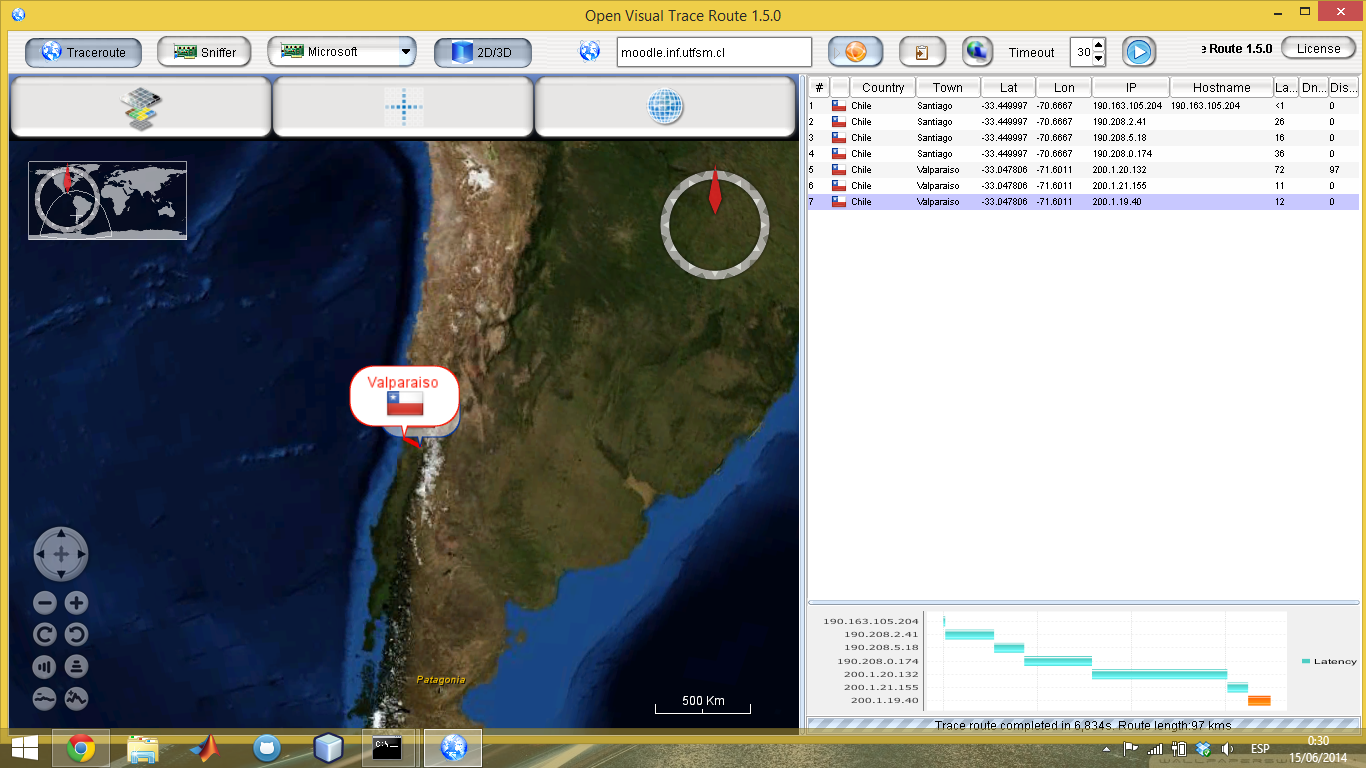
\includegraphics[width=1\textwidth]{moodle.png}
\caption{\label{fig:moodle}Traza para moodle.inf.utfsm.cl}
\end{figure}

\begin{figure}[H]
\centering
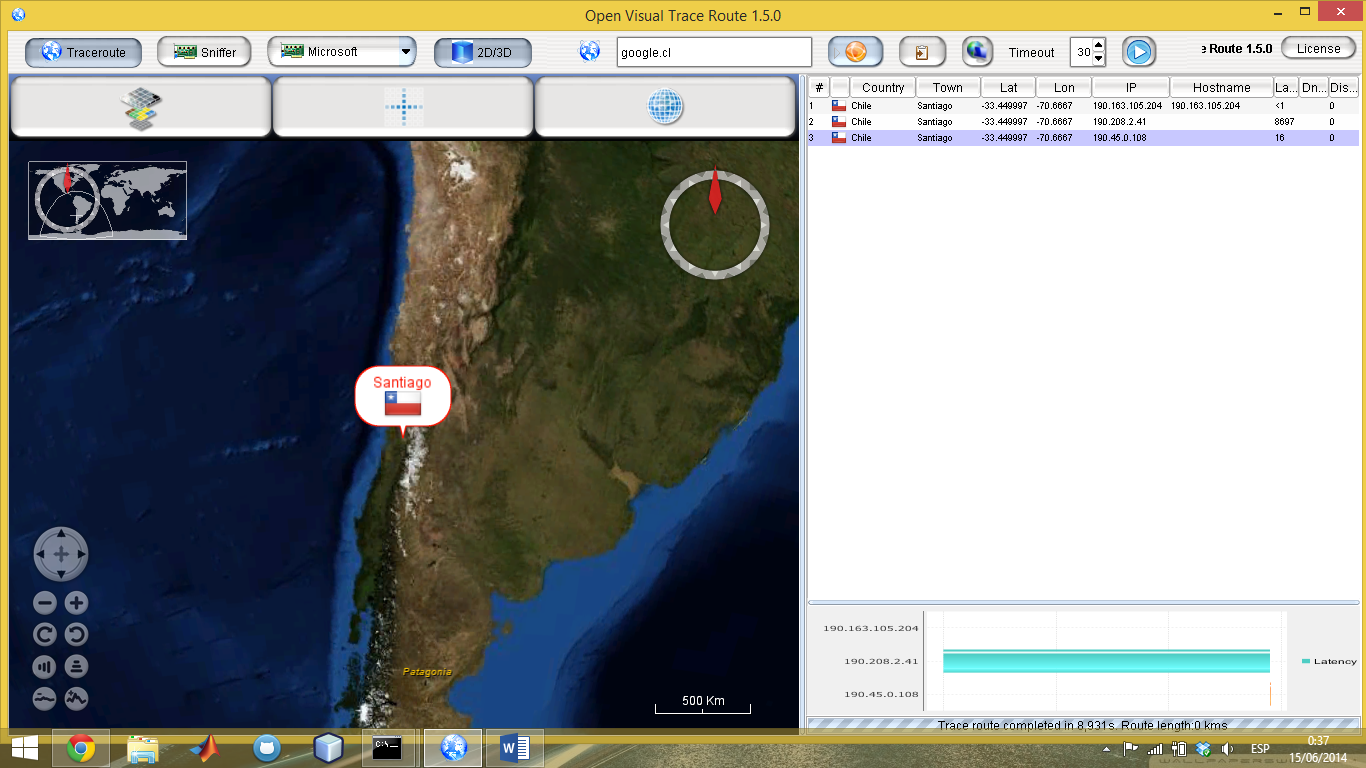
\includegraphics[width=1\textwidth]{google_cl.png}
\caption{\label{fig:google}Traza para google.cl}
\end{figure}

\begin{figure}[H]
\centering
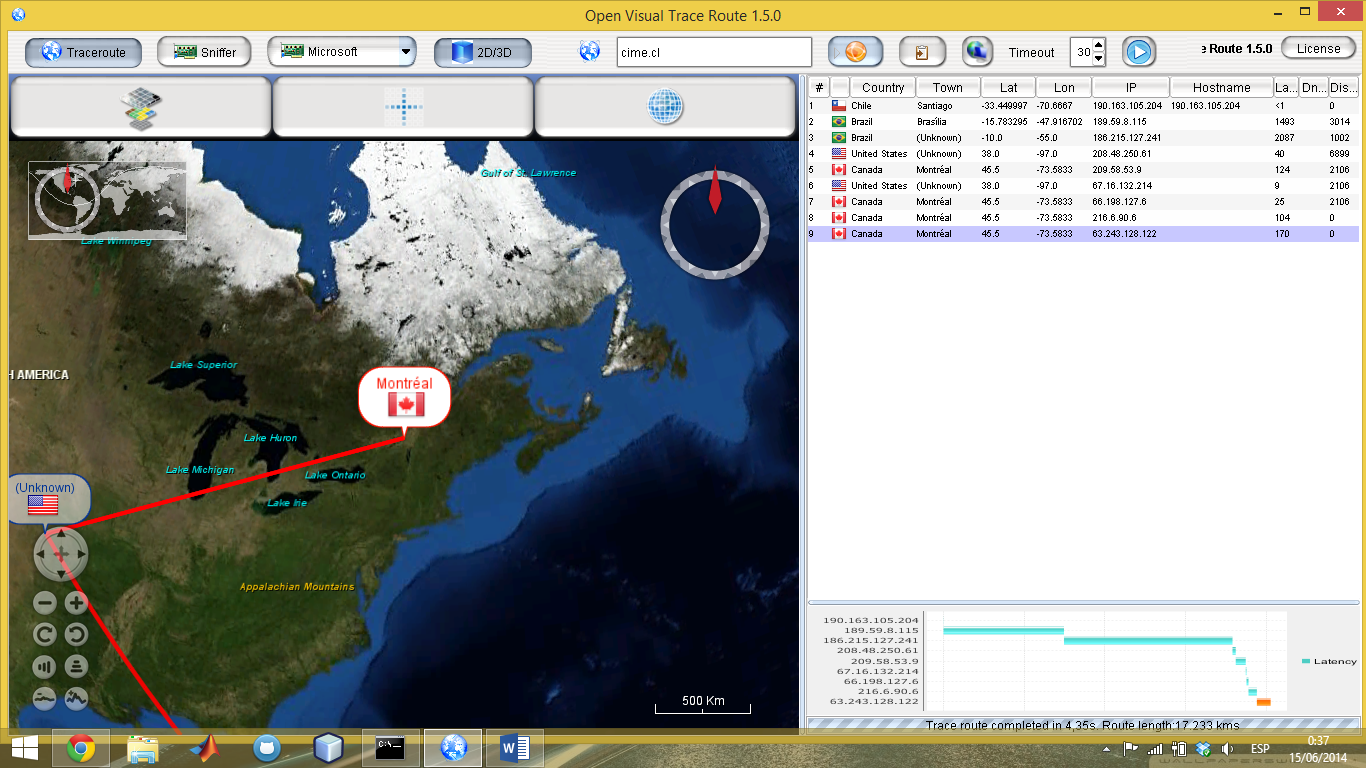
\includegraphics[width=1\textwidth]{cime_cl.png}
\caption{\label{fig:cime}Traza para cime.cl}
\end{figure}

\begin{figure}[H]
\centering
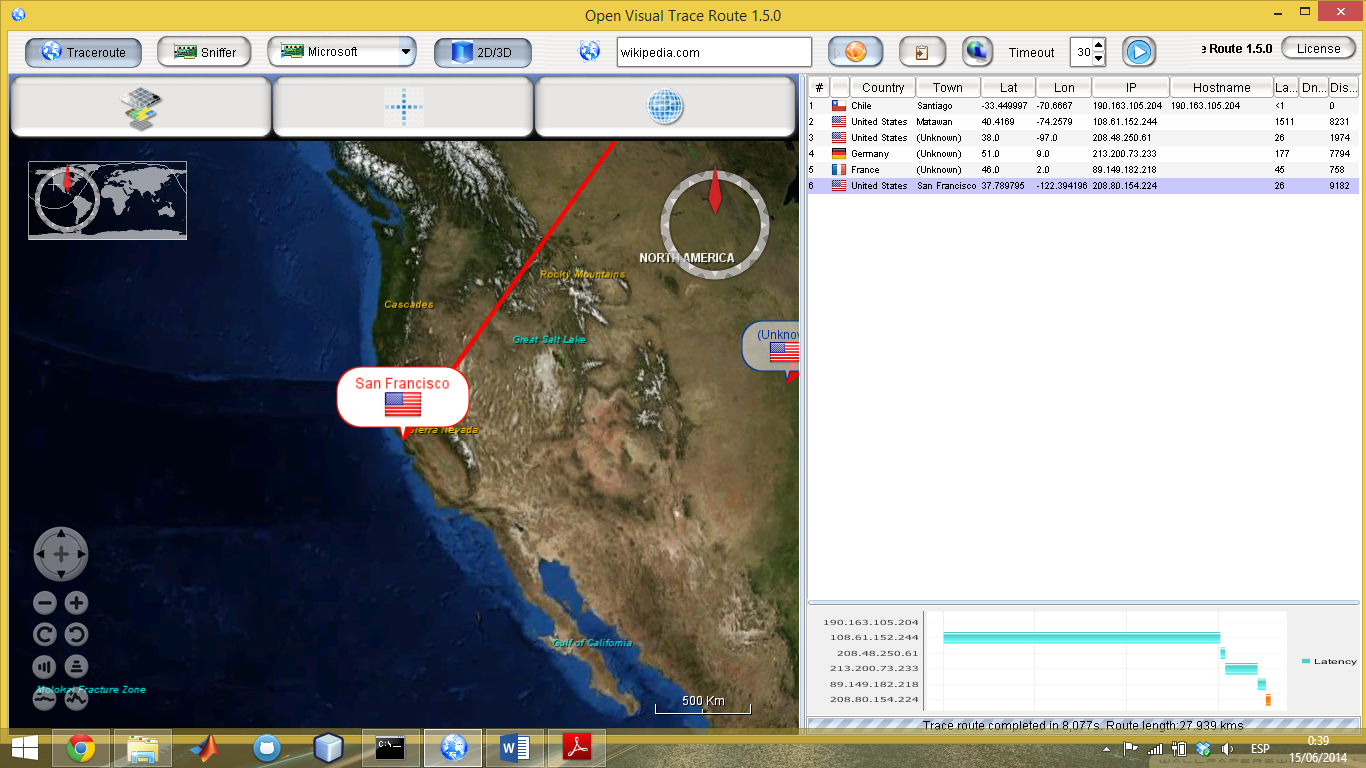
\includegraphics[width=1\textwidth]{wikipedia_com.png}
\caption{\label{fig:wikipedia}Traza para wikipedia.com}
\end{figure}

\begin{figure}[H]
\centering
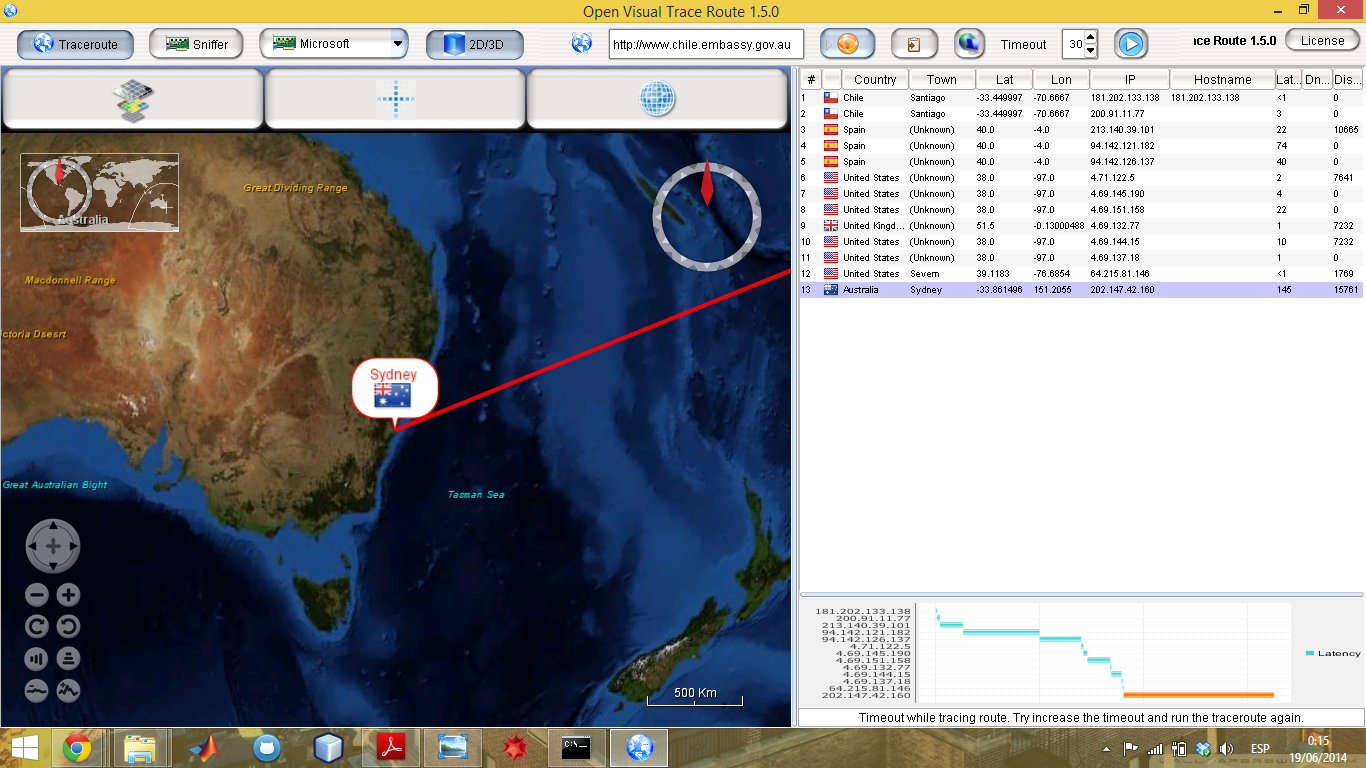
\includegraphics[width=1\textwidth]{embassy.png}
\caption{\label{fig:embassy}Traza para chile.embassy.gov.au}
\end{figure}

Como se puede visualizar en las imagenes, la ruta que siguen los paquetes varían entre una dirección a otra, mientras que unos sólo viajan dentro de Chile (como google.cl), hay otras que viajan a distintas partes del mundo. A continuación se explica brevemente como se establecen las rutas por las que viajan los paquetes via internet:\\

En el caso de que los paquetes viajen entre routers de un mismo AS de un ISP la ruta escogida, que aparece en el programa, es la obtenida mediante el protocolo de ruteo OSPF, que es el utilizado por la mayoria de los ISPs, a exepción de algunos casos como Cisco, que utiliza un protocolo privado. Este protocolo es del tipo link-state, y se encarga de encontrar el primer camino mas corto para enviar los paquetes a través de la red.\\

En el caso de que los paquetes tengan que viajar entre distintos ASs vía el backbone la ruta escogida se obtiene mediante el protoclo de ruteo BGP, este es un protocolo complejo el cual determina la ruta basándose en políticas de la red, o reglas que utilizan varios atributos de la ruta BGP.\\

Se puede observar que en al intentar encontrar la traza de la ruta seguida al visitar la página de la embajada de Australia, esta no termina y es abortada debido a que el timeout expiró. Esto ocurre debido a  que en algún punto de la ruta se filtra (via firewall, o por el mismo router) el payload del paquete UDP que contiene el ICMP Echo Request, que utiliza tracert en el SO de windows para saber que se llegó al host de destino. Sin embargo si utilizamos el comando traceroute en linux con la opcion -T, que utiliza paquetes TCP obtenemos el resultado completo.

\begin{figure}[H]
\centering
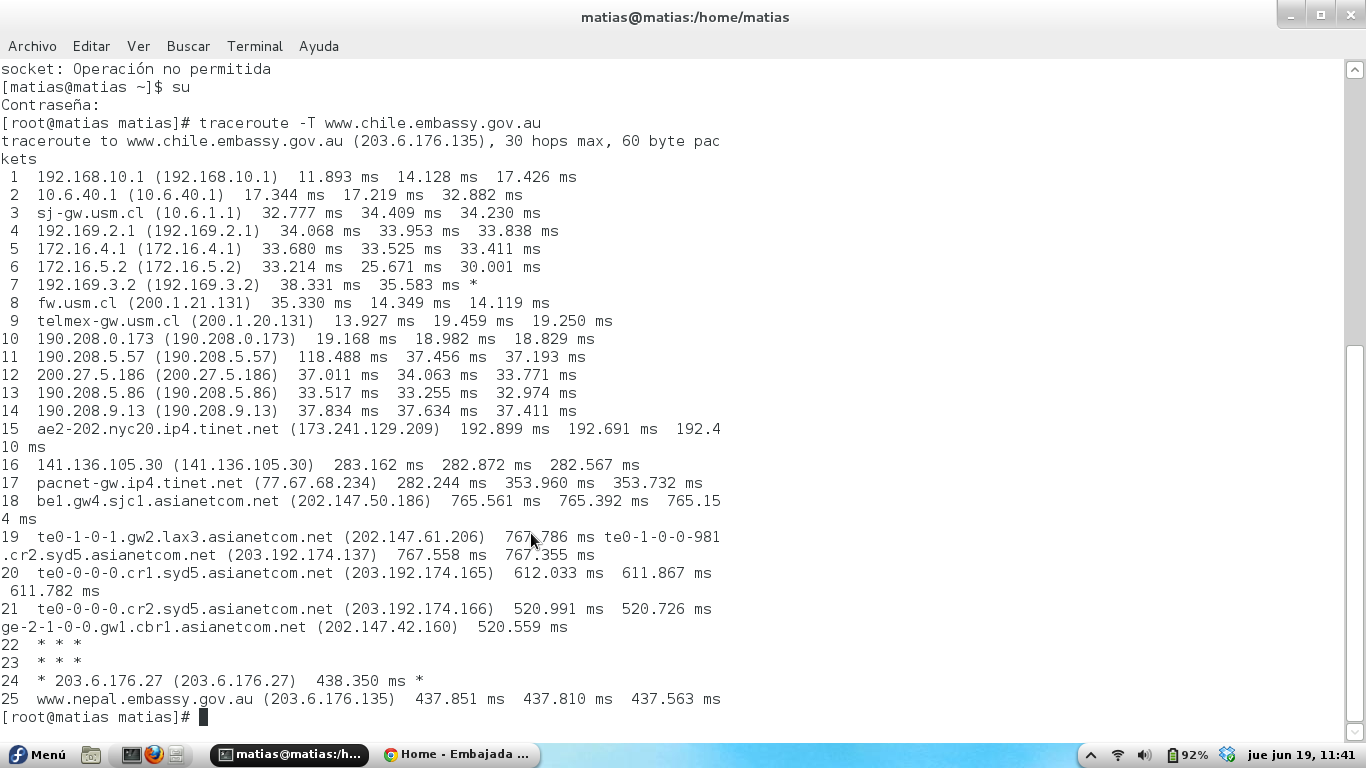
\includegraphics[width=1\textwidth]{tracerouteEmbassy.png}
\caption{\label{fig:Tembassy}Traza para chile.embassy.gov.au}
\end{figure}


\subsection{¿Como viajan los paquetes de un continente a otro?}
Hoy en día la información (paquetes) viajan de un continente a otro mediante conexiones submarinas compuestas de cables de fibra óptica, pero no siempre fué así. En sus inicios (1850) con la masificación del telégrafo, surgió la necesidad de conectar dos puntos separados por el mar Francia e Inglaterra. Fué así como se instaló el primer cable submarino, el cual estaba compuesto de cobre, sin embargo su calidad no era óptima, ya que las señales sufrían de retardos, que junto con la ausencia de blindaje en el cable, daba como resultado una señal irreconocible. Afortunadamente este cable sufrió un desperfecto un año después y así comenzó el desarrollo de una mejor solución técnica. Esta solución vino de Werner von Siemens quien desarrolló un recubrimiento para los cables que permitía su funcionamiento bajo el agua.\\

Con el paso de los años se desarrollaron nuevos tipos de cables, en los años 60 se desarrollaron los cables coaxiales, luego al llegar a la decada de los 80 ya se tenía planeado desplegar los siguientes cables submarinos con fibra óptica.\\

Hoy en día el 90\% del tráfico de internet, como se nombró anteriormente, circula a través  de estos cables de fibra óptica, estos tienen una gran potencia y pueden enviar mas de una señal a través de una misma fibra (gracias a DWDM). Estos cables se componen de un grupo de fibras ópticas, las cuales comparten espacio con hiladuras de aramida que le otorgan resistencia a la tracción. La fibra óptica esta rodeada de 7 capas que desde el interior hacia el exterior son: Gel de Petroleo, tubo de cobre o aluminio, policarbonato, alumnio, cabe de alambres de acero, cinta de Mylar y polietileno.\\

La instalación de estos cables se hace mediante barcos especializados conocidos bajo el nombre de barcos cableros, la ruta escogida para su instalación es estudiada profundamente y se escoje la mas segura (en terreno) y corta en la distancia del trayecto. Cuando uno de estos cables sufre un desperfecto estos mismos barcos son los encargados de reemplazar la parte averiada por una nueva (dicho de una manera simple, ya que en la realidad es una ardua tarea).\\

Estos cables recorren largas distancias, es por esto que para que la señal no se atuenue y se pierda se utilizan repetidores que están separados entre sí unos 100 km, frente a aproximadamente 1,5 km en los sistemas eléctricos. Los amplificadores ópticos recientemente desarrollados pueden aumentar todavía más esta distancia.

\begin{figure}[H]
\centering
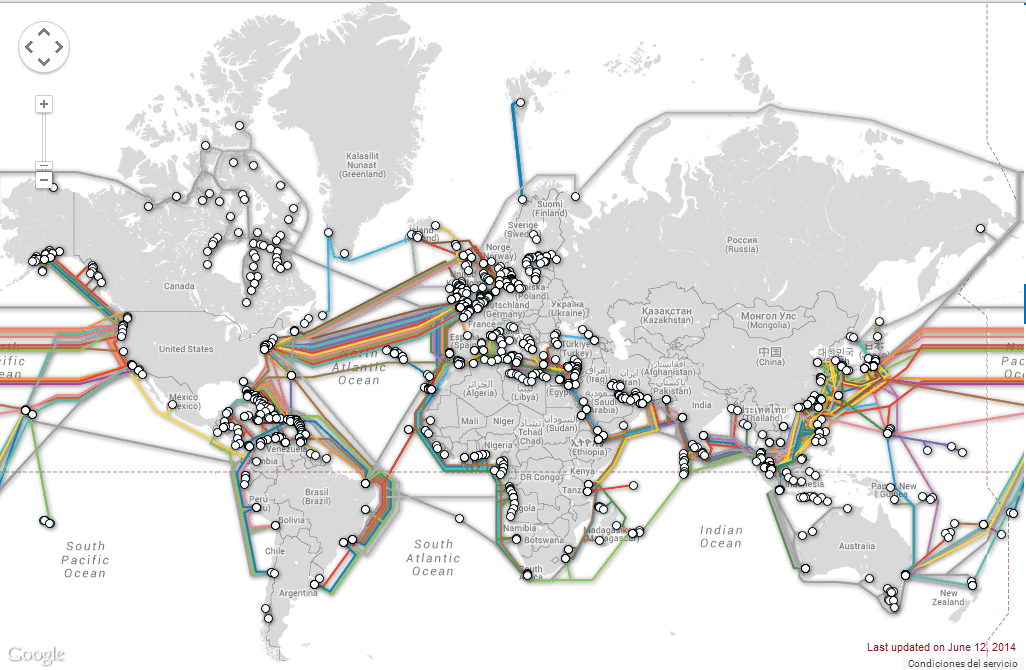
\includegraphics[width=0.7\textwidth]{Mapa_del_cableado_submarino.PNG}
\caption{\label{fig:mapa}cables submarinos instalados al 2014}
\end{figure}

~\\

\subsection{Enlaces internacionales de internet Chile}

A continuación se presentan los 3 enlaces que tiene Chile para contectarse al exterior:

\begin{itemize}

\item\textbf{Cable submarino Panamericano(PanAm):} Cable de fibra óptica que conecta Latino America con el Caribe, es usado por el lado oeste de Sudamérica, funciona a una velocidad de 70 Gbps. El anillo del pacífico (el cual incluye Chile) tiene capacidad de 4 lambdas (aproximadamente 40 Gbps).

\begin{figure}[H]
\centering
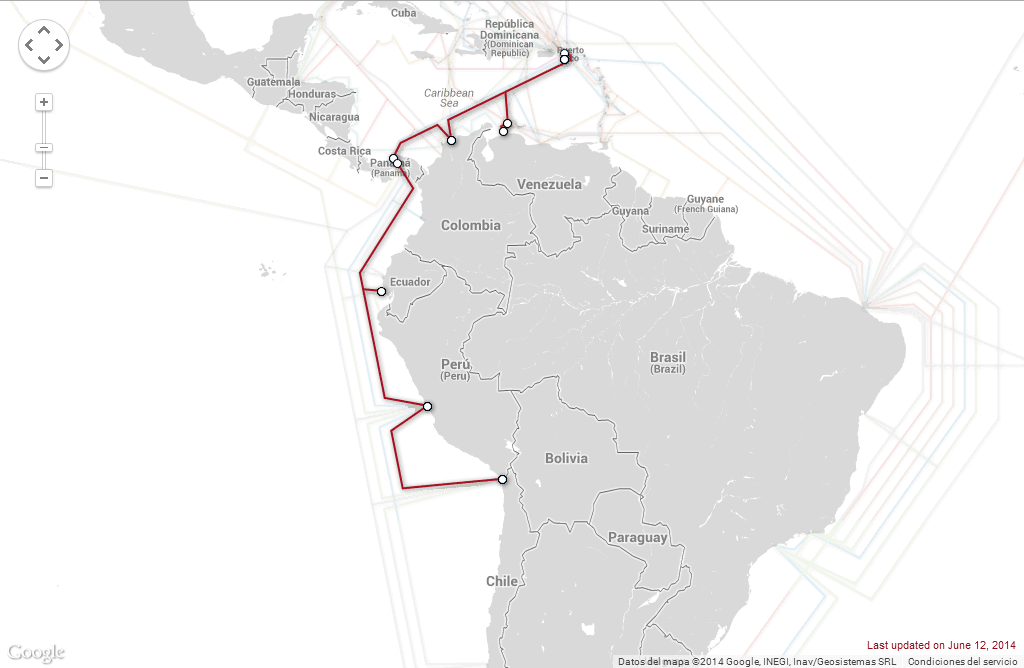
\includegraphics[width=0.5\textwidth]{PanAm.PNG}
\caption{\label{fig:PanAm} Cable de fibra óptica PanAm}
\end{figure}

\item\textbf{Sur América 1(Sam-1):} Cable de fibra óptica que conecta a Chile con Estados Unidos, Brasil, Puerto Rico, Argentina, Perú Guatemala y Colombia.

\begin{figure}[H]
\centering
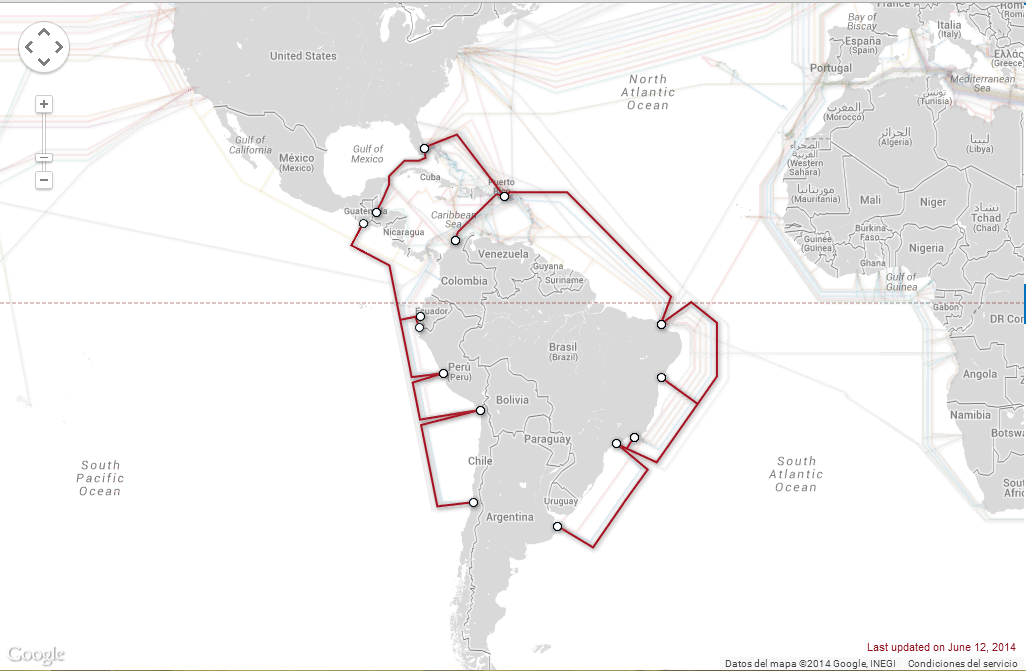
\includegraphics[width=0.5\textwidth]{Sam1.PNG}
\caption{\label{fig:Sam} Cable de fibra óptica Sam-1}
\end{figure}

~\\[4.0cm]

\item\textbf{South American Crossing (SAC)/Latin American Nautilus (LAN):} Cable de fibra óptica que rodea a toda Sudamérica, tiene una velocidad de 3.84 Tbps.

\begin{figure}[H]
\centering
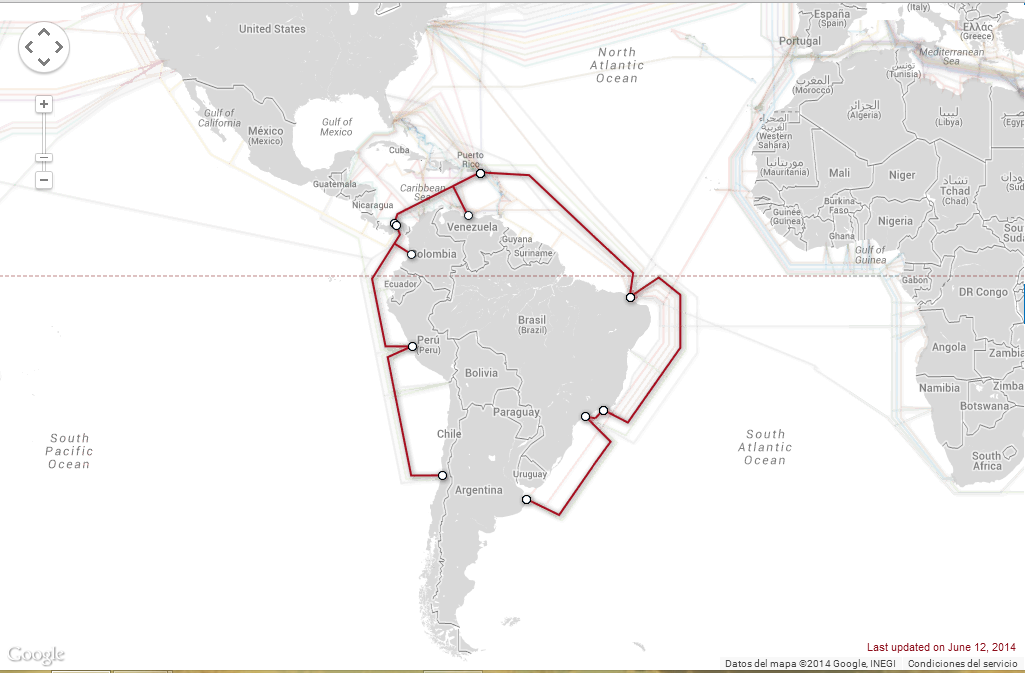
\includegraphics[width=0.5\textwidth]{Nautilus.PNG}
\caption{\label{fig:SAC/LAN} Cable de fibra óptica SAC/LAN}
\end{figure}

\end{itemize}

\end{document}